%%Created by Richard Balson
%%%%%%%%%%%%%%%%%%%%%%%%%%%%%%%%%%%%%%%%%%%%%%%%%%%%%%%%%%%%%

%------------------------------------------------------------
%
\documentclass{article}%
%Options -- Point size:  10pt (default), 11pt, 12pt
%        -- Paper size:  letterpaper (default), a4paper, a5paper, b5paper
%                        legalpaper, executivepaper
%        -- Orientation  (portrait is the default)
%                        landscape
%        -- Print size:  oneside (default), twoside
%        -- Quality      final(default), draft
%        -- Title page   notitlepage, titlepage(default)
%        -- Columns      onecolumn(default), twocolumn
%        -- Equation numbering (equation numbers on the right is the default)
%                        leqno
%        -- Displayed equations (centered is the default)
%                        fleqn (equations start at the same distance from the right side)
%        -- Open bibliography style (closed is the default)
%                        openbib
% For instance the command
%           \documentclass[a4paper,12pt,leqno]{article}
% ensures that the paper size is a4, the fonts are typeset at the size 12p
% and the equation numbers are on the left side
%
\usepackage{amsmath}%
\usepackage{amsfonts}%
\usepackage{amssymb}%
\usepackage{graphicx}
\usepackage{hyperref}
\usepackage[round]{natbib}
\usepackage{geometry}
\usepackage{color}
\usepackage{setspace}
\usepackage{pdfsync}
\usepackage{subfig}
%\usepackage{caption}
%\usepackage{subcaption}
\doublespacing

\def\imagetop#1{\vtop{\null\hbox{#1}}}

%-------------------------------------------
\newenvironment{proof}[1][Proof]{\textbf{#1.} }{\ \rule{0.5em}{0.5em}}

\geometry{top=3cm,bottom=3cm,left=2.5cm,right=3.5cm}

% \newcommand\iref{\textcolor{red}{ref}}
\newcommand\red{\textcolor{red}}

\graphicspath{{fig/}}

\hypersetup{colorlinks,linkcolor=black,filecolor=black,urlcolor=black,citecolor=black} 

\newcommand{\rich}[1]{\textcolor{green}{#1}}
\newcommand{\dean}[1]{\textcolor{blue}{#1}}

\title{Tracking Physiological Changes in an In-Vivo Model of Epilepsy: A Model-Based Approach}
\date{\today}
\author{Richard S. Balson, Dean R. Freestone, Anthony N. Burkitt, Mark J. Cook \\ and David B. Grayden}

\begin{document}
\maketitle

\section{Introduction}

\red{Estimate model parameters from a neural mass model of the hippocampus.}

\red{To improve the understanding of epilepsy} 

\red{How has this been achieved previously?}

\red{Introduction to neural mass model, freeman, jansen etc}

\red{What is the output of the model and why}

\red{Is a neural mass model a good model}

\red{Inadequacy of jansen model and intro to the wendling model}

\red{This model is capable of replicating key characteristics observed in EEG prior to and during seizure.}

\red{Is the Wendling model a good model}

\red{Previous work on estimating the neural mass model of the hippocampus has been done using a genetic algorithm.}

\red{Estimation of the neural mass model (Genetic Algorithm)}

\red{Kalman filter}

\red{Why the Kalman filter}

\red{What is being done, and why is it better or different?}

\red{What is being done with the UKF}

\red{Structure of the paper}

\red{Model estimation and accuracy for real data}

\section{Methods}

\subsection{Animal Model of Epilepsy}

In this study we make use of an \textsl{in vivo} model of temporal lobe epilepsy. In particular, we consider the tetanus toxin model of temporal lobe epilepsy, where the hippocampus is the seizure focus. This particular model was chosen as it has a localised seizure focus, and results in the animals having seizure events that are similar in terms of electrophysiology and clinical aspects to human patients with temporal lobe epilepsy. 

For this particular \textsl{in vivo} model, Sprague Dawley rats that weigh between 300-400 grams are used, with the approval of an ethics committee. Tetanus toxin is injected into the hippocampus at the location of -3.5mm anterior-posterior (AP), 3mm medial lateral and -3.5mm dorsal ventral (DV). This location is within the CA3 region of the hippocampus (Figure~\ref{fig: TetLoc}). Two depth electrodes are placed in the same location to record local field potentials from the seizure focus. A further three burr holes are made, one over the cerebellum, and two over the right hemisphere of the brain. Three electrodes are placed in the burr holes: the cerebellar electrode is used as a reference for all differential recordings, and the two electrodes over the right hemisphere are used to record local filed potentials from the surface of the brain. These electrodes are then connected to a pedestal and held in place by dental cement. The animals are left to recover for seven days, and are then recorded from 24 hours a day for six weeks.

 

\red{ What we are doing in this paper}


\subsection{Neural Mass Model} 

All neural field models can be described by a temporal and spatial response curve, and a function that relates membrane potentials to firing rates. For neural mass models the spatial element is removed from this general description such that

\begin{equation}\label{eq:conv_eq}
    v_n(t) = \frac{\alpha_{mn}}{\tau_{mn}}\int_{-\infty}^t  h_{mn}(t-t')g(v_m(t')) \,\mathrm{d}t' + v_r,
\end{equation}
where $\alpha_{mn}$ is a measure of the connectivity and synaptic strength between populations $m$ and $n$, $h_{mn}(t)$ is the temporal response curve, commonly referred to as a post synaptic response kernel, $\tau_{mn}$ is the time constant which indicates the average prorogation delay between populations $m$ and $n$ and $v_r$ is the resting membrane potential. The temporal response curve is a time delayed exponential decay function:
\begin{equation}
    h_{mn}(t) = \eta(t)t\exp\left(-\frac{t}{\tau_{mn}}\right),
\end{equation}
where $\eta(t)$ is the Heaviside step function. An example of a post synaptic response kernel can be seen in Figure~\ref{fig: Simple}


The firing rate of each population is determined from an asymmetric sigmoid activation curve. The sigmoid function translates the membrane potential of a population to its effective firing rate.
\begin{align}\label{eq:sigmoid}
    g\left(v_n(t)\right) =& \frac{1}{1+\exp{\left(\varsigma_n\left(v_{0n} - v_n(t)\right)\right)}}.
\end{align}
The quantity $\varsigma_n$ describes the gradient of the sigmoidal activation function and $v_{0n}$ the membrane potential that results in half the maximum firing rate. The constant $v_{0n}$ is a lumped parameter, that includes the effect of the resting membrane potential on the activation curve. An example of the sigmoidal activation function is demonstrated in Figure~\ref{fig: Simple}.

 \dean{Write something about $v_r$ being lumped into $v_0$.}

The convolution in Equation~\ref{eq:conv_eq} can also be written as the ordinary differential equation (ODE)
\begin{equation}\label{eq:2ndOrder}
    \mathrm{D}v_n(t) = \frac{\mathrm{d}^2 v_n(t)}{\mathrm{d}t^2} + \frac{2}{\tau_{mn}}\frac{\mathrm{d} v_n(t)}{\mathrm{d}t} + \frac{1}{\tau_{mn}^2} v_n(t) = \frac{\alpha_{mn}}{\tau_{mn}} g(v_m(t)),
\end{equation}
where $\mathrm{D}$ is a differential operator. Equation~\ref{eq:2ndOrder} can be written as two partial differential equations
\begin{equation} \label{eq:2ndOrderNMM}
    \frac{\mathrm{d} v_n(t)}{\mathrm{d}t} = z_n(t),\,\,\,\,\,    \frac{\mathrm{d}z_n(t)}{\mathrm{d}t} = \frac{\alpha_{mn}}{\tau_{mn}} g(v_m(t)) - \frac{2}{\tau_{mn}}z_n(t) - \frac{1}{\tau_{mn}^2} v_n(t),
\end{equation}
where $z_n(t)$ is the time derivative of $v_n(t)$. This forms the basis of a state-space model for all neural masses.

The simplest possible neural mass model is one that takes an input firing rate, and outputs a firing rate. A model of this is shown in Figure~\ref{fig: Simple}, where the effect of both the post synaptic response kernel and the sigmoidal activation curve are demonstrated.

\begin{figure}
	\centering
		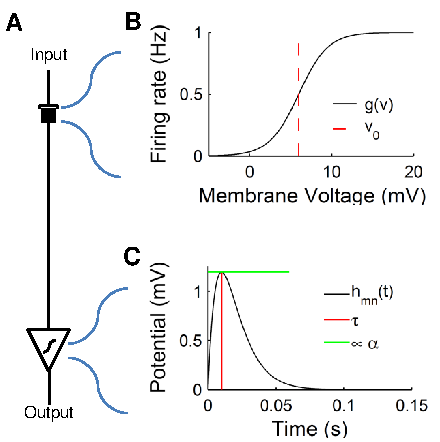
\includegraphics{Biological_Response.pdf}
	\caption{Simple Neural Mass Model. (\textbf{A}) An example of a simple neural mass model. This model consists of a single neural population - the triangle - and a single synapse - the square block. (\textbf{B}) Temporal response curve for a synapse. The black line demonstrates the response of a synapse to an impulse response. The time constant ($\tau$) and synaptic gain ($\alpha$) are demonstrated in this figure. The peak response of this function is $\alpha \exp(-1)$ and the time at which this peak occurs is equal to $\tau$. \textbf{C} Somatic response curve. The black line indicates the function $g(v)$ which is a sigmoidal activation curve. This function demonstrates the resulting normalized firing rate produced by a neural population as a function of the membrane potential over it. In this figure $v_{0}$ is the membrane potential at which the firing rate produced is half its maximum.}
	\label{fig: Simple}
\end{figure}

 \begin{figure}
 	\centering
 		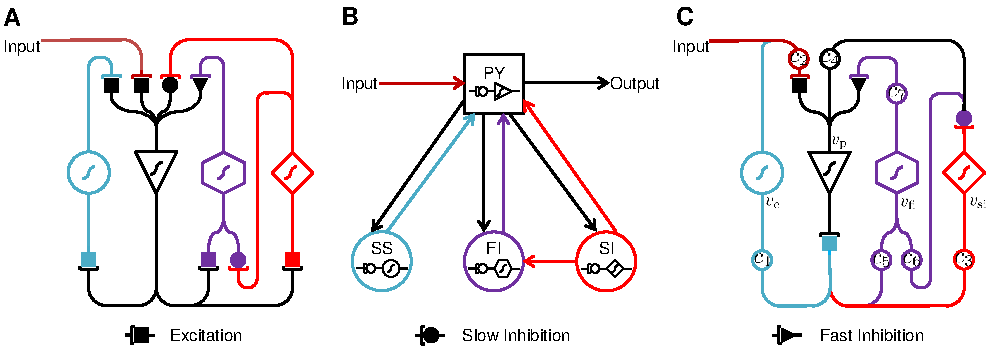
\includegraphics{fig/Biological_Model.pdf}
 	\caption{Graphical Description of the Neural Mass Model of the Hippocampus. (\textbf{A}) Graphical Description of the neural mass model of the hippocampus. }
 	\label{fig: Biological}
 \end{figure}


\subsection{Estimation}

\red{Generic description on a nonlinear system}

\red{Introduction to the UKF}

\red{The unscented filter}


\red{How states are predicted using the unscented transform}

\red{Definition of slow state matrix and its dynamics}

\red{Intialisation of UKF for stationary parameters}

 \begin{figure}
 	\centering
 		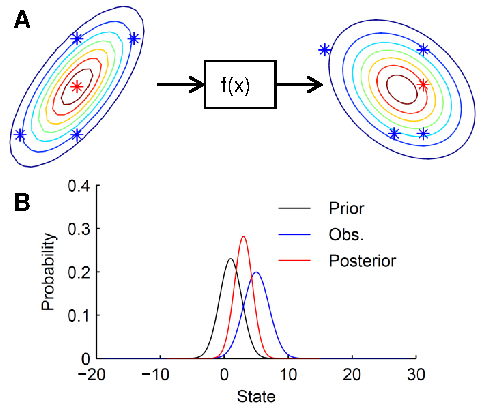
\includegraphics{fig/UnscentedKalman.pdf}
 	\caption{The unscented Kalman filter.}
 	\label{fig: Biological}
 \end{figure}

\red{Intialisation of UKF for varying parameters}

\red{Estimation of model input mean}

\red{Robustness test}

\section{Results}

\begin{figure}
 	\centering
 		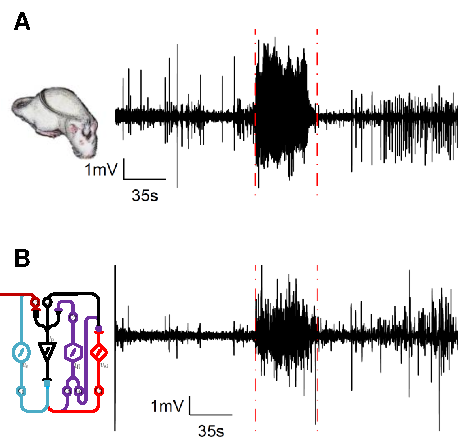
\includegraphics{fig/EEG.pdf}
 	\caption{Recorded and Simulated EEG.}
 	\label{fig: EEG}
 \end{figure}

\begin{figure}
 	\centering
 		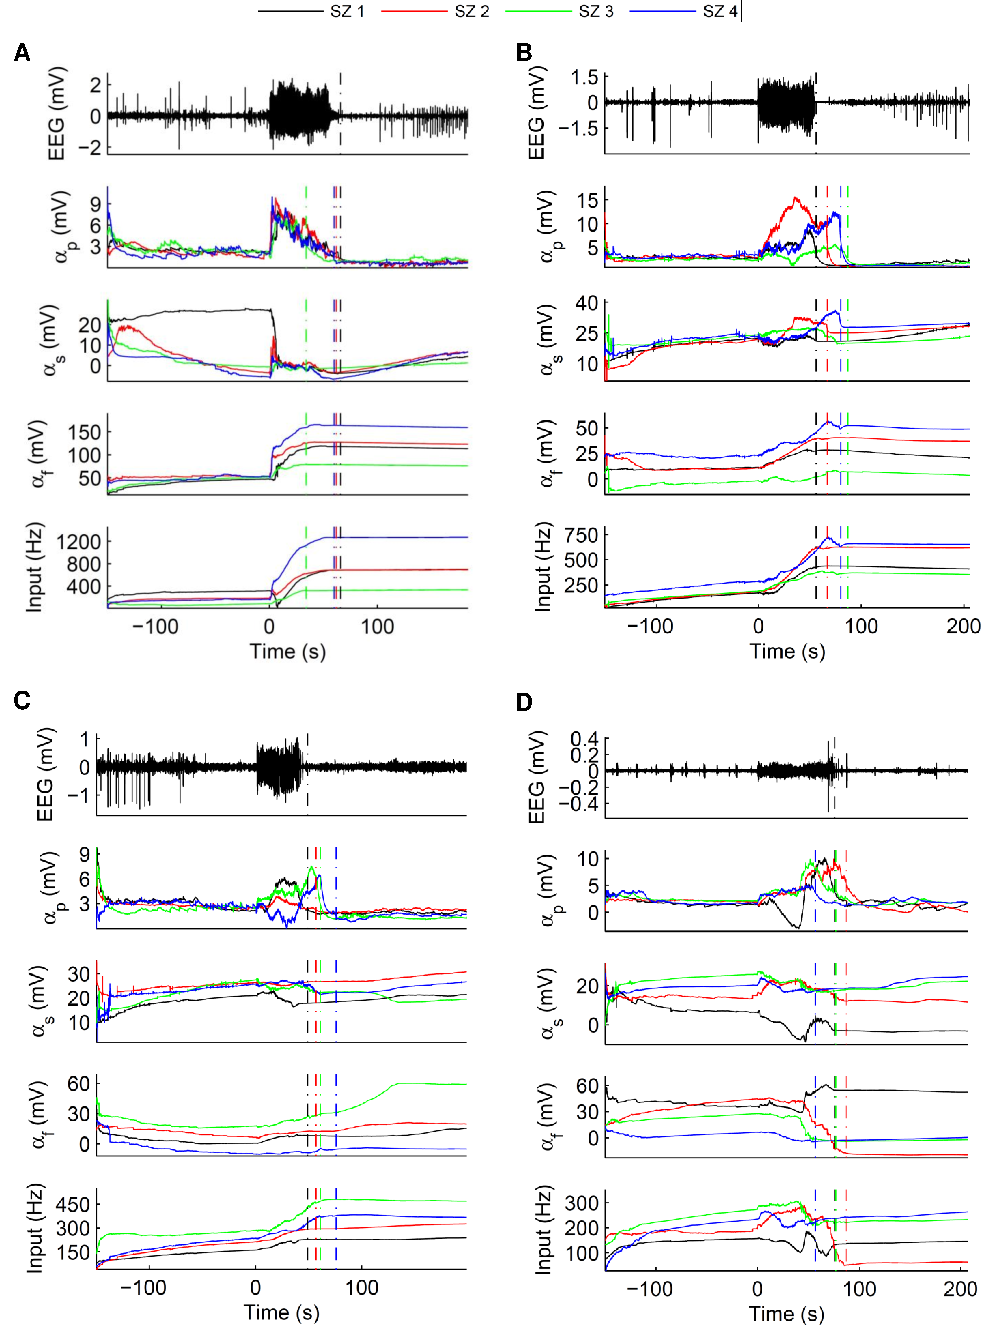
\includegraphics{fig/EstimationResults.pdf}
 	\caption{Estimation Results.}
 	\label{fig: EstimationResults}
 \end{figure}

\section{Discussion}

\red{Why estimation}

\red{Effect of stochastic input}

\red{Estimation of model parameters}

\red{Initialisation error}

\red{Observation Noise}

\red{Parameters varying}

% 
% \section{Discussion}


% 
% \section{Conclusion}

In this paper we have demonstrated that the tracking of neural dynamics using an unscented Kalman filter is feasible. We have also shown that there are clear differences between the mechanisms involved in seizure initiation and termination between and in some cases within animals. This information could be used to help with the development of new therapies. Some of the aspects that were not discussed in this paper include variability due to severity of seizures, and the long term evolution of seizures in an animal model where seizure frequency decreases over time. 
% 
% \section{Appendix}
\label{sec: AppendixA}

The reduction of the Wendling model is based on the principles of linear superposition. First notice that each synapse is a linear lowpass filter (equation~\ref{eqn: LaplaceNMM}). In figure~\ref{fig: Biological} there are eight such synapse. However, notice that numerous of these synapse have identical synaptic gains, and are connected by different connectivity constants. Given that for a linear system it is known that
\begin{align}
f(a\mathbf{x}) = af(\mathbf{x}),
\end{align} where $f(\cdot)$ is an arbitrary function, and $a$ is a constant. Therefore, the model can be simplified by moving the synapse closer to the respective populations. The result of this process is demonstrated in figure~\ref{fig: BiologicalMin}.

\begin{figure}  %%%%%%%%%%%%%%%%%%%%%%%%%%%%%%%%%%%%%%%
	\centering
		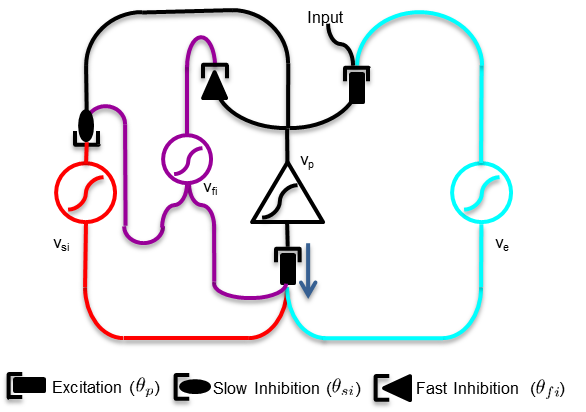
\includegraphics{Biological_Model_DescriptionMin.png}
	\caption{Graphical Description of the Wendling model (Minimised). Membrane potentials are shown and named $v_{b}$ where $b$ is $p$, $e$, $fi$ and $si$ for pyramidal, excitatory and slow and fast inhibitory populations, respectively. The synaptic gains of each population are specified by $\theta_{m}$ where $m$ is defined in the same manner as the membrane potentials and $\theta_{p}=\theta_{e}$. Each triangle and circle indicates a neural population. In particular, the triangle shape indicates the pyramidal population and the circle shapes represent interneurons. The triangles and circles model the action of the soma for the neural populations, and convert membrane potentials to firing rates. The synapses convert the firing rates to membrane potentials. Lastly, each line indicates a neural connection, which is specified by a connectivity constant.}
	\label{fig: BiologicalMin}
\end{figure}%%%%%%%%%%%%%%%%%%%%%%%%%%%%%%%%%%%%%%%%%%%%%

Now consider the full set of original model equations that would be required to specify figure~\ref{fig: Biological}
\begin{align}
\label{eqn: Fullmodel Descrip}
\mathrm{d}v_{po*}(t)&= z_{po*}(t)\mathrm{d}t\\
\mathrm{d}z_{po*}(t)&=\left(\frac{\theta_{p}(t)}{\tau_{p}}c_{1}g(v_{p}(t))-2\frac{z_{po*}(t)}{\tau_{p}}-\frac{v_{po*}(t)}{\tau_{p}^{2}}\right)\mathrm{d}t\\
\mathrm{d}v_{p1*}(t)&= z_{p1*}(t)\mathrm{d}t\\
\mathrm{d}z_{p1*}(t)&=\left(\frac{\theta_{p}(t)}{\tau_{p}}c_{3}g(v_{p}(t))-2\frac{z_{p1*}(t)}{\tau_{p}}-\frac{v_{p1*}(t)}{\tau_{p}^{2}}\right)\mathrm{d}t\\
\mathrm{d}v_{p2*}(t)&= z_{p2*}(t)\mathrm{d}t\\
\label{eqn: Pyr}
\mathrm{d}z_{p2*}(t)&=\left(\frac{\theta_{p}(t)}{\tau_{p}}c_{5}g(v_{p}(t))-2\frac{z_{p2*}(t)}{\tau_{p}}-\frac{v_{p2*}(t)}{\tau_{p}^{2}}\right)\mathrm{d}t\\
\label{eqn: SI}
\mathrm{d}v_{p3*}(t)&= z_{p3*}(t)\mathrm{d}t\\
\mathrm{d}z_{p3*}(t)&=\left(\frac{\theta_{si}(t)}{\tau_{si}}c_{4}g(v_{si}(t))-2\frac{z_{p3*}(t)}{\tau_{si}}-\frac{v_{p3*}(t)}{\tau_{si}^{2}}\right)\mathrm{d}t\\
\mathrm{d}v_{p4*}(t)&= z_{p4*}(t)\mathrm{d}t\\
\label{eqn: SI1}
\mathrm{d}z_{p4*}(t)&=\left(\frac{\theta_{si}(t)}{\tau_{si}}c_{6}g(v_{si}(t))-2\frac{z_{p4*}(t)}{\tau_{si}}-\frac{v_{p4*}(t)}{\tau_{si}^{2}}\right)\mathrm{d}t\\
\label{eqn: FI}
\mathrm{d}v_{p5*}(t)&= z_{p5*}(t)\mathrm{d}t\\
\label{eqn: FI2}
\mathrm{d}z_{p5*}(t)&=\left(\frac{\theta_{fi}(t)}{\tau_{fi}}c_{7}g(v_{fi}(t))-2\frac{z_{p4*}(t)}{\tau_{fi}}-\frac{v_{p5*}(t)}{\tau_{fi}^{2}}\right)\mathrm{d}t\\
\label{eqn: Exc}
\mathrm{d}v_{p6*}(t)&= z_{p6*}(t)\mathrm{d}t\\
\mathrm{d}z_{p6*}(t)&=\left(\frac{\theta_{e}(t)}{\tau_{e}}c_{2}g(v_{e}(t))-2\frac{z_{p6*}(t)}{\tau_{e}}-\frac{v_{p6*}(t)}{\tau_{e}^{2}}\right)\mathrm{d}t\\
\mathrm{d}v_{p7*}(t)&= z_{p7*}(t)\mathrm{d}t\\
\label{eqn: WienerFull}
\mathrm{d}z_{p7*}(t)&=\left(\frac{\theta_{p}(t)}{\tau_{p}}\mu -2\frac{z_{p7*}(t)}{\tau_{e}}-\frac{v_{p7*}(t)}{\tau_{p}^{2}}\right)\mathrm{d}t + \frac{\theta_{p}(t)}{\tau_{p}}\epsilon(t)\mathrm{d}W.\\
\end{align} In these equations $dW$ represents a Wiener process and is required as $\epsilon(t)\sim N(0,\sigma)$, where $\sigma$ and $\mu$ (equation~\ref{eqn: Wiener}) describe the mean and variance of the stochastic model input. Further, $v_{po}(t) $ and $v_{p1-7*}(t)$ represent the membrane potential produced by each synapse and $z_{po*}(t) $ and $z_{p1-7*}(t)$ their derivatives. The inputs to each neural population are specified by $v_{b}(t) $ and $z_{b}(t) $, and are the membrane potential of the specific population, where $b$ takes the values of $p$, $e$, $fi$ and $si$ representing pyramidal, excitatory, and slow and fast inhibitory populations, respectively. Therefore $v_{p}(t) $ is the output of the model. All $v_{b}(t) $ can be described in terms of $v_{po}(t)$ and $v_{p1-7}(t)$ as follows
\begin{align}
\label{eqn: pop1}
v_{p}(t) &= v_{p6*}(t)+v_{p7*}(t)-v_{p3*}(t)-v_{p5*}(t)\\
\label{eqn: pop2}
v_{e}(t) &= v_{po*}(t)\\
\label{eqn: pop3}
v_{si}(t) &= v_{p1*}(t)\\
\label{eqn: pop4}
v_{fi}(t) &= v_{p2*}(t)-v_{p4*}(t).
\end{align} Notice that equations~\ref{eqn: Fullmodel Descrip}-\ref{eqn: Pyr} and equations~\ref{eqn: SI}-\ref{eqn: SI1} are identical except for the connectivity constants. Further, in this model it is assumed that 
\begin{align}
\theta_p = \theta_e\\
\tau_p = \tau_e.
\end{align} Therefore, equations~\ref{eqn: Exc}-\ref{eqn: WienerFull} are identical, but have different inputs. Next consider the effect of the states $v_{p0-7*}(t)$ and $z_{p0-7*}(t)$ on the model inputs. Note that since the effect of $v_{p6*}(t)$ and $v_{p7*}(t)$ are additive, they can be added prior to being passed through the linear filter since
\begin{align}
f{x} + f{y} = f{x+y},
\end{align} where f is defined above and $x$ and $y$ are arbitrary variables. Therefore equations~\ref{eqn: Exc}-\ref{eqn: WienerFull} can be simplified to the following:
\begin{align}
\mathrm{d}v_{p1}(t)&= z_{p1}(t)\mathrm{d}t\\
\label{eqn: Wiener1}
\mathrm{d}z_{p1}(t)&=\left(\frac{\theta_{e}(t)}{\tau_{e}}(\mu +n_{e}g(v_{e}(t))-2\frac{z_{p1}(t)}{\tau_{e}}-\frac{v_{p1}(t)}{\tau_{e}^{2}}\right)\mathrm{d}t + \frac{\theta_{e}(t)}{\tau_{e}}\epsilon(t)\mathrm{d}W.
\end{align}. By making this reduction the effect of both the excitatory population and the input have been incorporated in one potential. Therefore, $v_{p7*}(t)$ is no longer required in equations~\ref{eqn: pop1}. 

Next consider the equations that only have connectivity constants that are different. Notice that these connectivity constants scale the input to the function, and this scaling can be performed after the input is transformed by the linear function. Therefore, equations~\ref{eqn: Fullmodel Descrip}-\ref{eqn: Pyr} can be represented by a single equation such that
\begin{align}
\mathrm{d}v_{po}(t)&= z_{po}(t)\mathrm{d}t\\
\mathrm{d}z_{po}(t)&=\left(\frac{\theta_{p}(t)}{\tau_{p}}g(v_{p}(t))-2\frac{z_{po}(t)}{\tau_{p}}-\frac{v_{po}(t)}{\tau_{p}^{2}}\right)\mathrm{d}t.
\end{align} Notice that in doing this equations~\ref{eqn: pop2}-\ref{eqn: pop4} are no longer valid and need to be altered to include the connectivities that have been removed from their relevant functions
\begin{align}
\label{eqn: pop2n}
v_{e}(t) &= c_{1}v_{po}(t)\\
\label{eqn: pop3n}
v_{si}(t) &= c_{3}v_{p0}(t)\\
\label{eqn: pop4n}
v_{fi}(t) &= c_{5}v_{p0}(t)-v_{p4*}(t).
\end{align}. 

A similar argument can be applied to equations~\ref{eqn: SI}-\ref{eqn: SI1} which can be simplified to
\begin{align}
\mathrm{d}v_{p2}(t)&= z_{p2}(t)\mathrm{d}t\\
\mathrm{d}z_{p2}(t)&=\left(\frac{\theta_{si}(t)}{\tau_{si}}g(v_{si}(t))-2\frac{z_{p2}(t)}{\tau_{si}}-\frac{v_{p2}(t)}{\tau_{si}^{2}}\right)\mathrm{d}t.
\end{align} Again by doing so equation~\ref{eqn: pop1} and~\ref{eqn: pop4n} are no longer valid and become
\begin{align}
v_{p}(t) &= v_{p1}(t)-c_{4}v_{p2}(t)-v_{p5*}(t)\\
v_{fi}(t) &= c_{5}v_{p0}(t)-c_{6}v_{p2}(t).
\end{align}. Lastly for simplicity equations~\ref{eqn: FI}-\ref{eqn: FI2} are replaced with
\begin{align}
\mathrm{d}v_{p3}(t)&= z_{p3}(t)\mathrm{d}t\\
\label{eqn: FI1}
\mathrm{d}z_{p3}(t)&=\left(\frac{\theta_{fi}(t)}{\tau_{fi}}c_{7}g(v_{fi}(t))-2\frac{z_{p3}(t)}{\tau_{fi}}-\frac{v_{p3}(t)}{\tau_{fi}^{2}}\right)\mathrm{d}t.
\end{align} Which results in the set of equations demonstrated in the methods section. Notice that the $n_{b}$ term used in the general form of the equations specifies connectivities that were not removed from the full model description equations due to simplification.



\bibliographystyle{apalike}
\bibliography{RealData}


\end{document}

